% Copyright 2004 by Till Tantau <tantau@users.sourceforge.net>.
%
% In principle, this file can be redistributed and/or modified under
% the terms of the GNU Public License, version 2.
%
% However, this file is supposed to be a template to be modified
% for your own needs. For this reason, if you use this file as a
% template and not specifically distribute it as part of a another
% package/program, I grant the extra permission to freely copy and
% modify this file as you see fit and even to delete this copyright
% notice. 

\documentclass[english,aspectratio=169]{beamer}
% Replace the \documentclass declaration above
% with the following two lines to typeset your 
% lecture notes as a handout:
%\documentclass{article}
%\usepackage{beamerarticle}


% There are many different themes available for Beamer. A comprehensive
% list with examples is given here:
% http://deic.uab.es/~iblanes/beamer_gallery/index_by_theme.html
% You can uncomment the themes below if you would like to use a different
% one:
%\usetheme{AnnArbor}
%\usetheme{Antibes}
%\usetheme{Bergen}
%\usetheme{Berkeley}
%\usetheme{Berlin}
%\usetheme{Boadilla}
%\usetheme{boxes}
%\usetheme{CambridgeUS}
%\usetheme{Copenhagen}
%\usetheme{Darmstadt}
%\usetheme{default}
%\usetheme{Frankfurt}
\usetheme{Goettingen}
%\usetheme{Hannover}
%\usetheme{Ilmenau}
%\usetheme{JuanLesPins}
%\usetheme{Luebeck}
%\usetheme{Madrid}
%\usetheme{Malmoe}
%\usetheme{Marburg}
%\usetheme{Montpellier}
%\usetheme{PaloAlto}
%\usetheme{Pittsburgh}
%\usetheme{Rochester}
%\usetheme{Singapore}
%\usetheme{Szeged}
%\usetheme{Warsaw}

\usepackage[utf8x]{inputenc} % Allows Spanish tildes
\usepackage{graphicx} % Allows insert images
\graphicspath{ {fig/} }
\usepackage{ragged2e} % Allows text alignments
\usepackage{hyperref} % Allows hyperlinks
\usepackage{multicol} % Allows multiple columns
%\usepackage{wasysym} % Allows mars and venus symbols
\usepackage[english]{babel}
%\usepackage{xcolor}

%---------------------------------------------------------------------------------
%	TITLE PAGE
%---------------------------------------------------------------------------------

\title[NBpy]{NBpy: Network-based (R)Statistics in Python}

% A subtitle is optional and this may be deleted
%\subtitle{}

\author[]{Ljuba, Waleed, \& Zeus}
% - Give the names in the same order as the appear in the paper.
% - Use the \inst{?} command only if the authors have different
%   affiliation.


% - Use the \inst command only if there are several affiliations.
% - Keep it simple, no one is interested in your street address.

%\date{}
% - Either use conference name or its abbreviation.
% - Not really informative to the audience, more for people (including
%   yourself) who are reading the slides online

%\logo{\includegraphics[width=\textwidth]{}}

\subject{NBpy}
% This is only inserted into the PDF information catalog. Can be left
% out. 

% If you have a file called "university-logo-filename.xxx", where xxx
% is a graphic format that can be processed by latex or pdflatex,
% resp., then you can add a logo as follows:

% \pgfdeclareimage[height=0.5cm]{university-logo}{university-logo-filename}
% \logo{\pgfuseimage{university-logo}}

% Delete this, if you do not want the table of contents to pop up at
% the beginning of each subsection:
%\AtBeginSection[]
%{
%  \begin{frame}<beamer>{Contenidos}
%    \tableofcontents[currentsection]
%  \end{frame}
%}

% Let's get started
\begin{document}

\begin{frame}%1
  \titlepage

  \centering
  \vspace*{-0.5cm}
  
\includegraphics[width=\textwidth]{neurohack.png}
\end{frame}

%%%%%%%%%%%%%%%%%%%%%%%%%%%%%%%%%%%%%%%%%%%%%%%%%%%%%%%%%%%%%%%%%%
% Section
\section{Intro}

\begin{frame}{Context}%2
  \framesubtitle{Longitudinal brain networks}
  
  \centering
  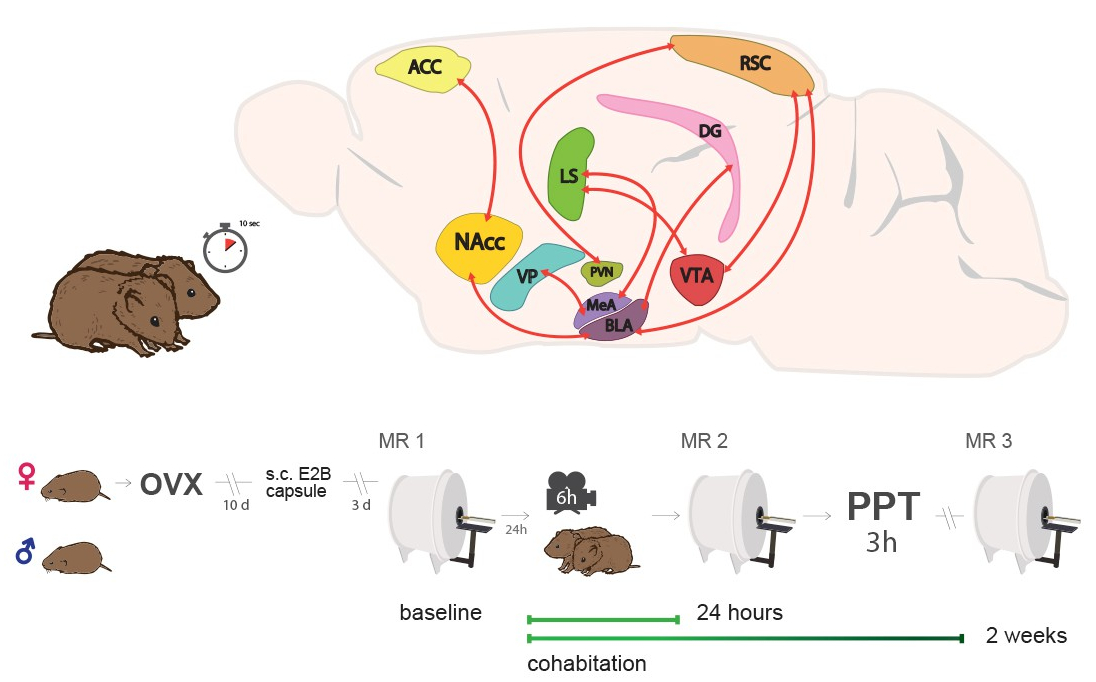
\includegraphics[width=.8\linewidth]{voles.jpg}\\[0.25cm]

  \raggedleft
  (López-Gutierrez et al., \textit{eLife}, 2021)

\end{frame}

\begin{frame}{Context}%3
  \framesubtitle{Prairie voles}
  
  \centering
  
\includegraphics[width=.8\linewidth]{rmvoles.jpeg}\\[0.25cm]

\end{frame}

% Section
\section{NBR}

\begin{frame}{Network Based Statistics framework}%4
  \centering
  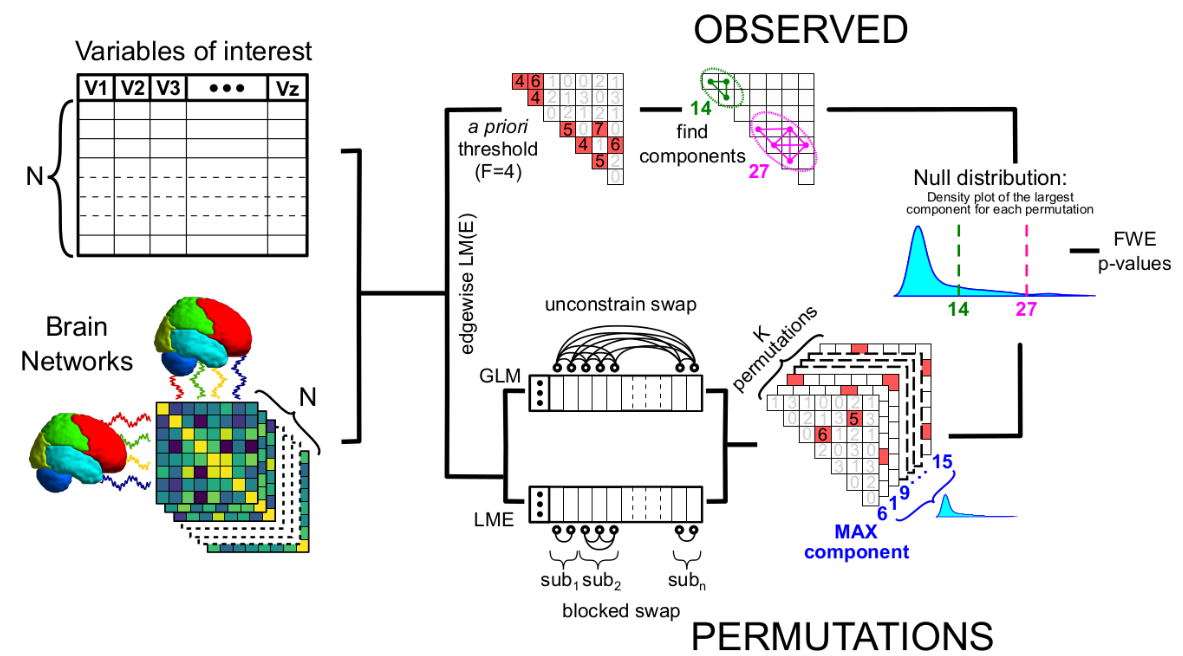
\includegraphics[width=\textwidth]{NBR.png}\\[0.1cm]
  
  \raggedright
  (Gracia-Tabuenca \& Alcauter, \textit{bioRxiv}, 2021)

\end{frame}

\begin{frame}{NBR}%5
  
  \large
  \begin{itemize}
    \item First CRAN release 0.1.2 (March 2020)
    \begin{itemize}
        \item \url{https://cran.r-project.org/package=NBR}
        \item $>$6k downloads (\url{https://cranlogs.r-pkg.org/badges/grand-total/NBR})
        \item Most mails from users ask about computing efficiency...
    \end{itemize}
  \end{itemize}

\end{frame}

\begin{frame}{Benchmarking}%6
  \centering
  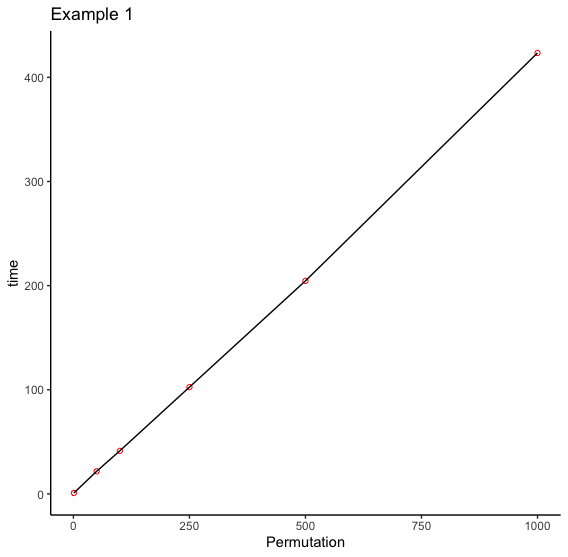
\includegraphics[width=\textwidth]{NBR_example1.png}\\[0.1cm]
  
\end{frame}


\end{document}
